 \let\negmedspace\undefined
\let\negthickspace\undefined
\documentclass[journal]{IEEEtran}
\usepackage[a5paper, margin=10mm, onecolumn]{geometry}
%\usepackage{lmodern} % Ensure lmodern is loaded for pdflatex
\usepackage{tfrupee} % Include tfrupee package

\setlength{\headheight}{1cm} % Set the height of the header box
\setlength{\headsep}{0mm}     % Set the distance between the header box and the top of the text

\usepackage{gvv-book}
\usepackage{gvv}
\usepackage{cite}
\usepackage{amsmath,amssymb,amsfonts,amsthm}
\usepackage{algorithmic}
\usepackage{graphicx}
\allowdisplaybreaks
\usepackage{textcomp}
\usepackage{xcolor}
\usepackage{txfonts}
\usepackage{listings}
\usepackage{enumitem}
\usepackage{mathtools}
\usepackage{gensymb}
\usepackage{comment}
\usepackage[breaklinks=true]{hyperref}
\usepackage{tkz-euclide} 
\usepackage{listings}
% \usepackage{gvv}                                        
\def\inputGnumericTable{}                                 
\usepackage[latin1]{inputenc}                                
\usepackage{color}                                            
\usepackage{array}                                            
\usepackage{longtable}                                       
\usepackage{calc}                                             
\usepackage{multirow}                                         
\usepackage{hhline}                                           
\usepackage{ifthen}                                           
\usepackage{lscape}
\begin{document}

\bibliographystyle{IEEEtran}
\vspace{3cm}

\title{1-1.5-27}
\author{AI24BTECH11002 - K.AKSHAY TEJA}
% \maketitle
% \newpage
% \bigskip
{\let\newpage\relax\maketitle}

\renewcommand{\thefigure}{\theenumi}
\renewcommand{\thetable}{\theenumi}
\setlength{\intextsep}{10pt} % Space between text and floats


\numberwithin{equation}{enumi}
\numberwithin{figure}{enumi}
\renewcommand{\thetable}{\theenumi}

\textbf{Question:}\\
Show that the points $\vec{P}=\myvec{-2\\3\\5},\vec{Q}=\myvec{1\\2\\3}$ and $\vec{R}=\myvec{7\\0\\-1}$ are collinear.
    

 \solution
 \begin{table}[h!]
	 \centering
	 \begin{tabular}{|c|c|}
	\hline
	Vector&Description\\
	\hline
	Vector A&  \(\hat{i} - 2 \hat{j} + 3 \hat{k}\)\\
	\hline
	Vector B& \(2\hat{i} +3 \hat{j} -4\hat{k}\)\\
	\hline
	Vector C& \(\hat{i} -3\hat{j} +\hat{k}\)\\
	\hline
\end{tabular}
 
	 \caption{Coordinates of points P,Q and R}
	 \label{tab:Coordinates}
\end{table}

Points $\vec{P},\vec{Q}$ and $\vec{R}$ are collinear if 
\begin{align}
	\text{rank}\myvec{\vec{P} & \vec{Q} & \vec{R}}^\top = 2\\[5pt]
	\implies \myvec{-2 & 3 & 5\\1 & 2 & 3\\7 & 0 & -1}\xleftrightarrow[]{R_2 \leftarrow 2R_2 + R_3} \myvec{-2 & 3 & 5\\0 & 7 & 11\\7 & 0 & -1}\\[5pt]
	\xleftrightarrow[]{R_3 \leftarrow 2R_3 + 7R_1} \myvec{-2 & 3 & 5\\0 &7 & 11\\0 & 21 & 33} \xleftrightarrow[]{R_3 \leftarrow R_3 - 3R_2} \myvec{-2 & 3 & 5\\0 & 7 & 11\\0 & 0 & 0}
\end{align}
\newpage
	\begin{figure}[h!]    
	  \begin{center}
		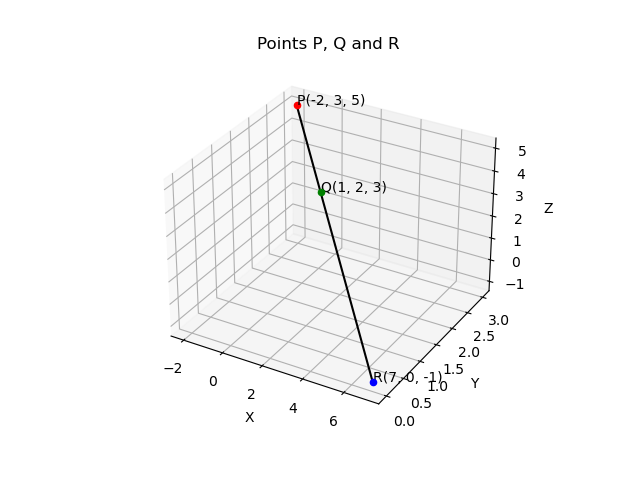
\includegraphics[width=0.7\textwidth]{fig/fig.png}
		\label{Graph}
		  \caption{Plot of points P, Q and R}  
	 \end{center}	  
	\end{figure}

\end{document}


